\documentclass{article}

\usepackage[a4paper, total={6in, 8in}]{geometry}
\usepackage[utf8]{inputenc}
\usepackage{fancyhdr}
\usepackage{graphicx}
\usepackage{enumitem}

\pagestyle{fancy}
\fancyhf{}
\lhead{John J Li}
\rhead{CSE360 Summer 2021 Notes}
\rfoot{\thepage}
\renewcommand{\headrulewidth}{0.4pt}

\setlength{\parskip}{1em}
\setlength\parindent{0px}
\title{CSE360 Summer 2021 Notes}
\date{\today}
\author{John J Li}

\begin{document}
    \section*{System Architecture}

    \subsection*{Architecture Design}

    \begin{itemize}
        \item Understading how a software system should be organized
        \item Designing the overall structure of the system
    \end{itemize}

    Often represented using simple block diagrams 
    \begin{itemize}
        \item High-level picture of the system structure
        \item Each block represents a component in the system 
        \item Arrows represent data or signals passed from one component to another 
    \end{itemize}

    The advantages: easy to understand. Disadvantages: too informal, doesn't show the type of 
    relationships among components or externally visible properties.

    % \begin{center}
    %     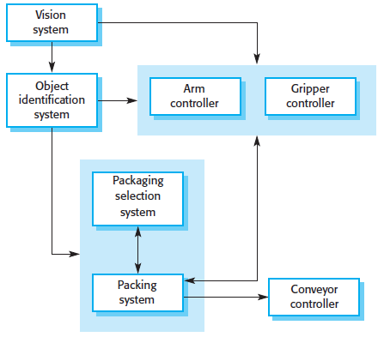
\includegraphics[scale=0.7]{block_diagram.png}
    % \end{center}
    
    \subsection*{Architectural Decision}

    \begin{itemize}
        \item How will the system be distributed across hardware cores and processors?
        \item What will be the fundamental approach used to structure the system? 
        \item What architectural pattern or syles might be used?
        \item How should the architecture of the system be documented?
    \end{itemize}

    % \begin{center}
    %     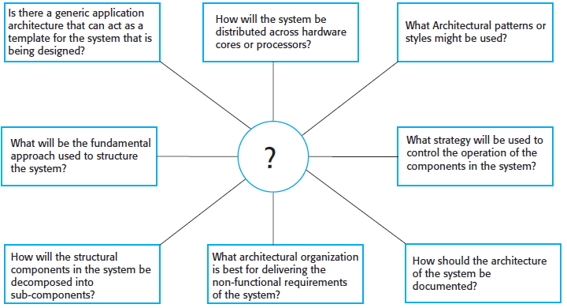
\includegraphics[scale=1]{architectural_decisions.png}
    % \end{center}

    \subsection*{4+1 View Model}

    \begin{itemize}
        \item Logical view 
        \begin{itemize}
            \item Key abstractions in the system as objects or object classes
            \item Relate system requirements to objects
        \end{itemize}
        \item Process view 
        \begin{itemize}
            \item How the system is composed of interacting processes
            \item Usingful for making judgement about non-functional requirements 
        \end{itemize}
        \item Development view 
        \begin{itemize}
            \item How the software is decomposed for development 
            \item Useful for software managers and programmers 
        \end{itemize}
        \item Physical view 
        \begin{itemize}
            \item How the system hardware and software components are distributed across 
            the processors in the system 
            \item Useful for system engineers 
        \end{itemize}
        \item +1 link all views through common use cases or scenarios 
    \end{itemize}

    % \begin{center}
    %     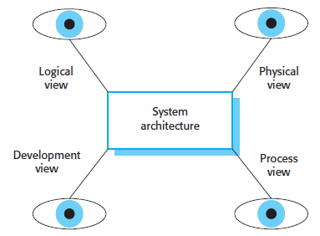
\includegraphics[scale=0.7]{4+1_View_model.png}
    % \end{center}

    \subsection*{Architectural Patterns}

    A pattern is a means for representing, sharing, and reusing knowledge; and it may be 
    represented using tabular and graphical descriptions.

    An architectural pattern is a stylized, abstract description of good design practice. 
    It has been tried and tested in diff environments and it should include info about 
    when they are and are not useful and the strengths and weaknesses.

    Examples:
    \begin{itemize}
        \item Model-View-Controller (MVC)
        \item Layered architecture 
        \item repository architecture 
        \item Client-server architecture 
        \item Pipe and filter architecture
    \end{itemize}

    \subsection*{Model-View-Controller}

    Often used for web applications and it splits the system into three different 
    components: Model - stores and manages data; View - GUI; Controller - 
    converts input from the View into demands to retrieve or update data from the 
    Model and passes info from Model to the View.

    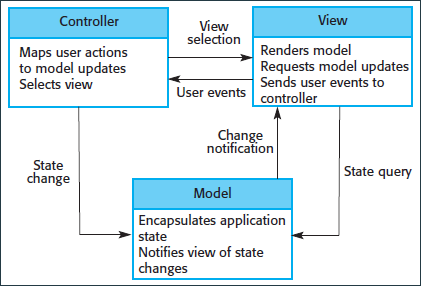
\includegraphics[scale=0.7]{model_view_controller.png}
    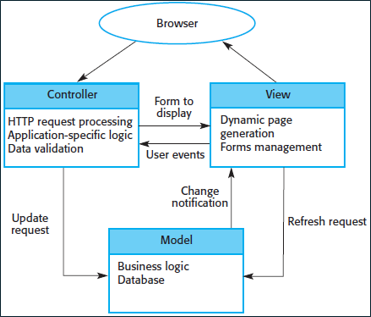
\includegraphics[scale=0.7]{model_view_controller-webbrowser.png}
    \begin{center}
        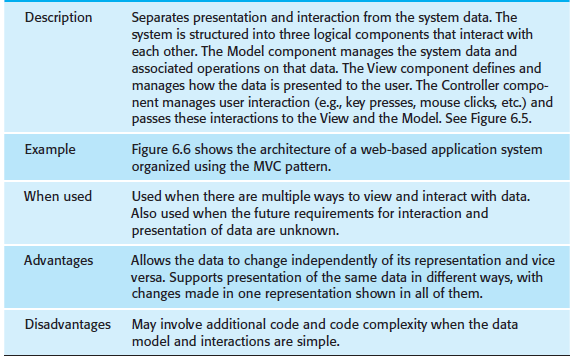
\includegraphics[scale=0.7]{model_view_controller-desc.png}
    \end{center}

    \subsection*{Layered Architecture}    

    Used to model the interfacing of the subsystems and it supports incremental dev 
    of subsystems in diff layers. When a layer interface changes, only the adjacent layers
    are affected. 
    The number of layers is arbitrary.

    \begin{center}
        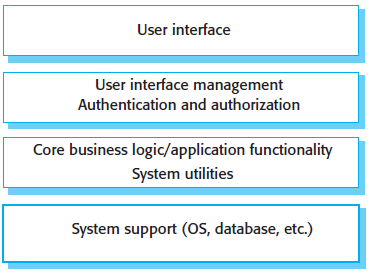
\includegraphics[scale=0.7]{layered_architecture.png}
        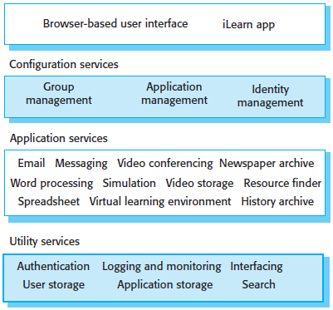
\includegraphics[scale=0.7]{layered_architecture-example.png}
        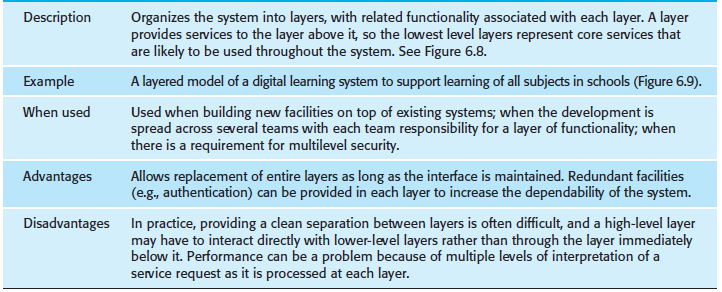
\includegraphics[scale=0.7]{layered_architecture-desc.png}
    \end{center}

    \subsection*{Repository Architecture}

    Subsystems must exchange data which can be done by storing datat in central database
    and which can be accessed by all subsystems or each subsystem maintains its own 
    database and passes data to other subsystems. When large amounts of data need to be 
    shared, the repository model is most commonly used.

    \begin{center}
        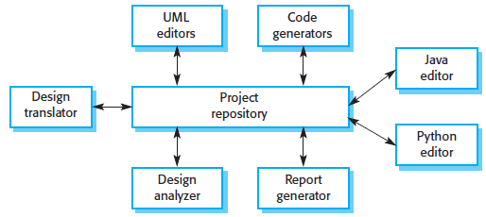
\includegraphics[scale=0.7]{repository_architecture.png}
        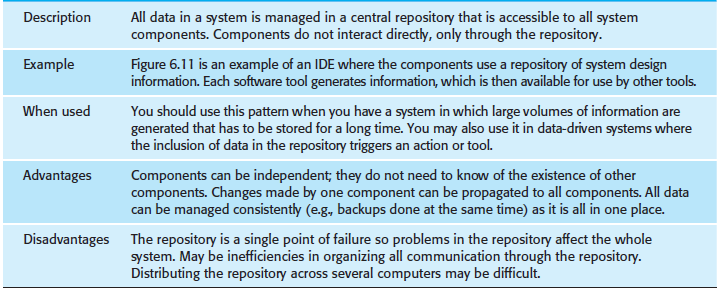
\includegraphics[scale=0.7]{repository_architecture-desc.png}
    \end{center}

    \subsection*{Client-Server Architecture}

    Distributed system model which shows how data and processing is distributed across 
    a range of components. It is a set of stand-alone servers, a set of clients, and a 
    network to connect the two.

    \begin{center}
        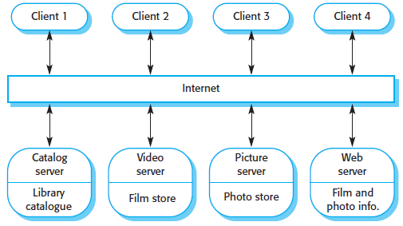
\includegraphics[scale=0.7]{client-server_architecture.png}
        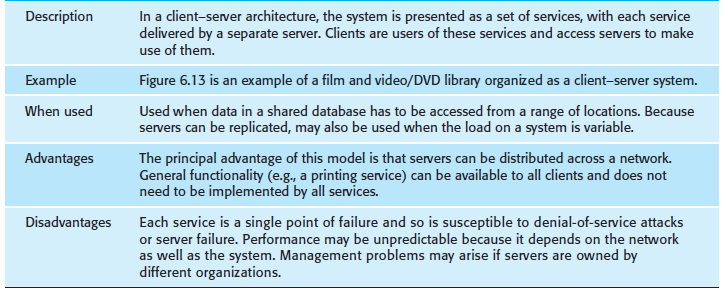
\includegraphics[scale=0.7]{client-server_architecture-desc.png}
    \end{center}

    \subsection*{Pipe and Filter Architecture}

    Data comes into a process, gets transformed and the resulting output is used as the 
    input for the next process. Not a good choice for interactive systems.

    \begin{center}
        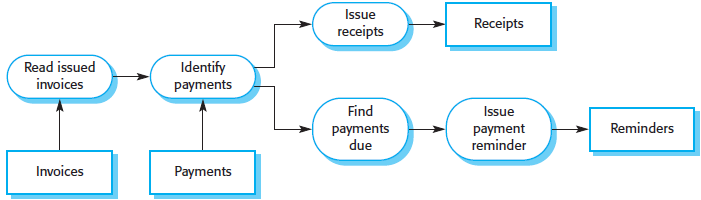
\includegraphics[scale=0.7]{pipe_and_filter_architecture.png}
        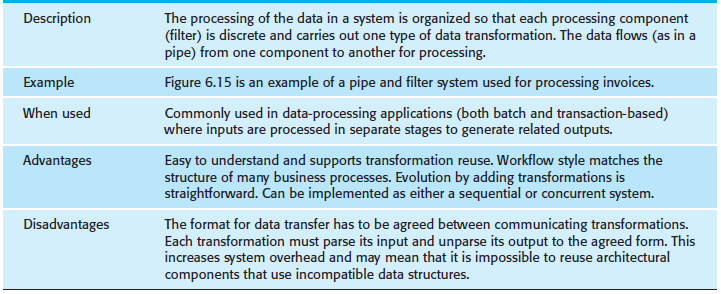
\includegraphics[scale=0.7]{pipe_and_filter_architecture-desc.png}
    \end{center}

    \section*{Design Patterns}
    
    \subsection*{Architecture vs Design}

    Software architecture gives the high-levvel organization of the software and it 
    identifies the main structural components in a system and the relationships between 
    them.

    Sofware design gives the code-level design and it identifies what each class doing, 
    their relationships and scope.

    \subsection*{Design patterns}

    A patter is a description of the problem and the essence of its solution. A design 
    pattern is a way of reusing abstract knowledge about a problem and its solution. 

    It should have High cohesion and low coupling.

    \subsection*{Cohesion}

    Cohesion is the degree of interaction within a module.

    There are 7 levels:
    \begin{itemize}
        \item Functional (best): all essential elements for a single task is in one module 
        \item Sequential 
        \item Communicational 
        \item Procedural 
        \item Temporal 
        \item Logical 
        \item Coincidental (worst): Elements have no conceptual relationship other than the 
        location in the source code. 
    \end{itemize}

    % \begin{center}
    %     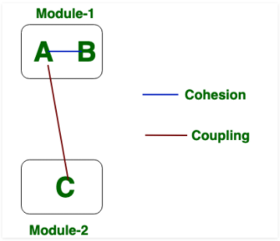
\includegraphics[scale=0.7]{cohesion.png}
    % \end{center}

    \subsection*{Coupling}

    Coupling is the degree of interaction between modules.

    There are 5 levels:
    \begin{itemize}
        \item Data (best): modules are independent from each other and communication by 
        only passing data 
        \item Stamp 
        \item Control 
        \item Common 
        \item Content (worst): a module can modify the data of another module.
    \end{itemize}

    \subsection*{Encapsulation}

    Def: Hides the details from everything; is the process to contain information.

    Implementation: variables of a class are private and functions are public so other 
    classes can get and set the data.

    \begin{center}
        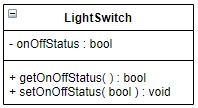
\includegraphics[scale=0.7]{encapsulation.png}
    \end{center}

    \subsection*{Abstraction}

    Def: Shows only what is needed and hides the unwanted info. It is the process to gain 
    info.

    Implementation: Create an abstract class and extend to show more info or add complexity.

    \begin{center}
        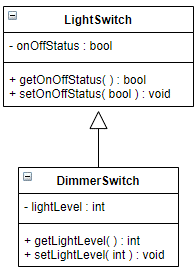
\includegraphics[scale=0.7]{abstraction.png}
    \end{center}

    \subsection*{Design Problems and Patterns}

    To use patterns in your design, you need to recognize that any design problem may have 
    an associated pattern that can be applied.

    There is three catagory: Creational patterns which is focused on creating objects; 
    Structural patterns which setups the relationship between objects; Behavioral patterns 
    which defins how objects interact with each other.

    Examples: 
    \begin{itemize}
        \item Iterator 
        \begin{itemize}
            \item Provide a standard way of accessing the elements in a collection,
            irrespective of how that collection is implemented.
        \end{itemize}
        \item Facade
        \begin{itemize}
            \item Tidy up the interfaces to a number of related objects that have often been 
            developed incrementally
        \end{itemize}
        \item Observer
        \begin{itemize}
            \item Tell several objects that the state of some other objects has changed 
        \end{itemize}
        \item Decorator
        \begin{itemize}
            \item Allow for possibility of extending the functionality of an existing class at 
            run-time
        \end{itemize}
    \end{itemize}

    \section*{Project Management}

    Focused on making sure the software is delievered on time and is built in accordance 
    with the requirements. Always needed b/c software dev is always subject to budget and 
    software contraints.

    \subsection*{Project success criteria}

    Important goals of project management for most engineering projects:
    \begin{itemize}
        \item Deliver software to the customer at the agreed time
        \item Keep overall costs within budget
        \item Deliver software that meets the customer’s expectations
        \item Maintain a coherent and well-functioning development team
    \end{itemize}

    \subsection*{Software project differences}

    The product is intangible and software projects are often "one-off" projects. Software 
    processes are variable and org specific.

    Factors influencing project management:
    \begin{itemize}
        \item Company size
        \item software Customers
        \item software size
        \item software type
        \item org culture 
        \item software dev processes
    \end{itemize}

    \subsection*{Project management activities}

    Project planning
    \begin{itemize}
        \item Project manager are responsible for planning, estimating, and scheduling 
        project dev and assigning tasks to people.
        \item Ensures the work is build to required standards and monitor progress to check
        dev is on time and within budget
    \end{itemize}

    Risk management 
    \begin{itemize}
        \item Project managers assess the risks that may affect the project, monitor the 
        risks, and take action when the problems arise.
    \end{itemize}

    People management 
    \begin{itemize}
        \item Project managers choose people for their team and establish ways of working 
        that lead to effective team performance.
    \end{itemize}

    Reporting
    \begin{itemize}
        \item Project managers report the progress of the project to customers and 
        managers of the company.
    \end{itemize}

    \subsection*{Risk management}

    \subsubsection*{Risk identification}
    \begin{itemize}
        \item Estimation 
        \item Organizational 
        \item People 
        \item Requirements 
        \item Tech 
        \item Tools
    \end{itemize}
    % \begin{center}
    %     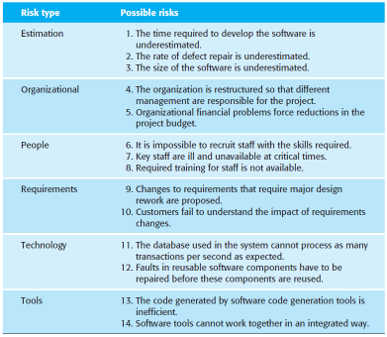
\includegraphics[scale=1]{risk_identification.png}
    % \end{center}

    \subsubsection*{Risk analysis}
    
    Need to choose the risks that are most significant and monitor them. Assess the 
    probability of a risk occuring and the lv of effect the risk may have on the 
    project.
    % \begin{center}
    %     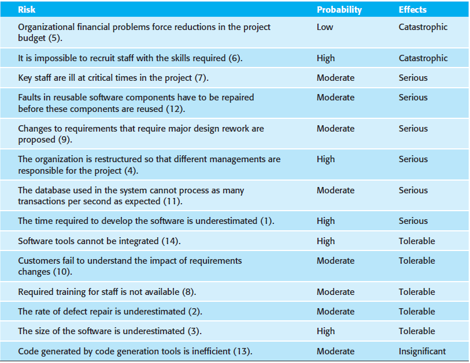
\includegraphics[scale=1]{risk_analysis.png}
    % \end{center}

    \subsubsection*{Risk planning}

    Need to ask "what-if" questions: What if the performance of open-source software is 
    inadequate? What if an economic downturn leads to budget cuts? etc.

    Develop strategies to manage these risks: Avoidance: reduce the chance of 
    them happening; minimization: reduce the impact; contingency: prepare for the worst and 
    have a plan to deal w/ it.

    \subsection*{Effort allocation}

    40-20-40\% rule: 40-50\% for front-end; 15-20\% for construction (coding); 30-40\% for 
    testing and installation.
    Some engineering managers believe more than 40\% of overall effort should be
    used for analysis and design.
    Some that use agile development say less time
    should be spent on the “front end” and more during the construction phase.

    \subsection*{Setting up a schedule}

    Common items needed:
    \begin{itemize}
        \item Define deliverables and milestones
        \item Identify tasks that belong to deliverables
        \item Identify relationships between deliverables and activities
        \item Determine type and size of resources needed to complete task
        \item Allocate people to activities
        \item Create a system to track the progress of each activity
    \end{itemize}

    \subsubsection*{Gantt Chart}

    \begin{center}
        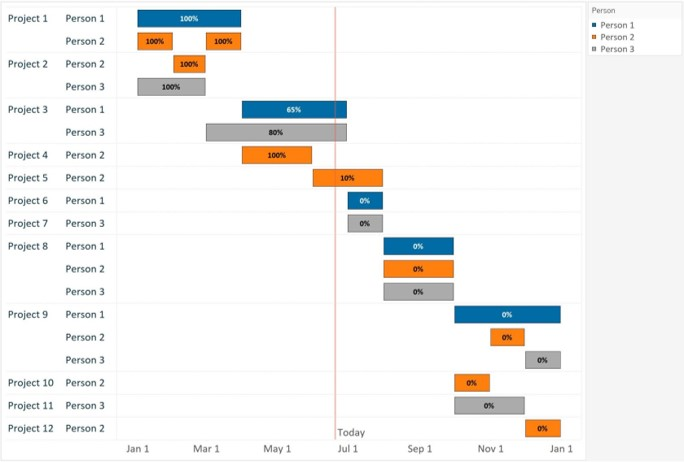
\includegraphics[scale=0.7]{gantt_chart.jpg}
    \end{center}

\end{document}